\documentclass[UTF8]{ctexart}
\usepackage{graphicx}
\usepackage{float}
\usepackage{geometry}
\usepackage{fancyhdr}
\usepackage{lastpage}
\usepackage{subfigure}
\usepackage{booktabs}
\geometry{left=2.54cm,right=2.54cm,top=3.18cm,bottom=3.18cm}%页边距
\pagestyle{fancy}
\lhead{\includegraphics[scale=1]{sjtu-logo-red.pdf}}  
\rhead{Intel与AMD处理器发展历程报告} 
\cfoot{第 \thepage\ 页\ 共 \pageref{LastPage} 页} 


\begin{document}

\begin{titlepage}
    \begin{center}
        \includegraphics[width=0.8\textwidth]{sjtu-name-blue.pdf}\\[1cm]
        \textsc{\Huge \bfseries 课程报告}\\[1.5cm]
        \includegraphics[width=0.3\textwidth]{sjtu-badge-blue.pdf}\\[0.5cm]

        \Huge \bfseries{Intel与AMD处理器发展历程报告}\\[1cm]
        \Large \bfseries{518021910971 裴奕博}
    \end{center}
\end{titlepage}

\tableofcontents
\newpage
\section{CPU发展概述}
1947年12月,由美国贝尔实验室的肖克利、巴丁和布拉顿组成的研究小组,发明了晶体管。这种新的材料工艺相比之前的真空电子管,体积小巧、无需预热、耗能极低,很快取代了电子管成为了新一代电子电路的首选。在随后的几十年间,伴随着集成电路的发明,由这种材料制成的电子电路规模越来越大。从小规模、中规模集成电路到大规模、超大规模集成电路。
\begin{figure}[H]
    \begin{center}
        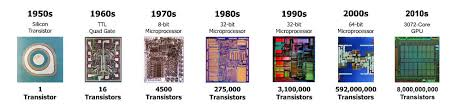
\includegraphics[width=0.8\textwidth]{figure/ICdev.jpg}
        \caption{集成电路的发展}
    \end{center}
\end{figure}
随着人类对计算机计算能力和便携性的要求不断提升,人们提出了“微型计算机”的概念,要实现这一点,首当其冲的就是将计算机的中央处理单元小型化。1971年,Intel公司制造出了第一个商用微处理器即4004,也宣告了第四代计算机时代的来临。从1971年至今的近50年间,随着个人计算机(PC)的成熟、发展和普及,作为计算机核心的CPU也得以迅猛发展。两家“本是同根生”的半导体公司,Intel和AMD,在这几十年间共同促成了CPU技术的不断提升,时至今日也是市面上处理器的最主流选择。本报告即梳理了从1971年至今,两家公司系列处理器的发展历程。
\newpage
\section{Intel系列处理器发展历程}
1968年创立的Intel,是全球目前收入和市值最高的半导体公司。1971年,Intel的工程师发明了世界上第一款CPU4004。在之后的几十年间,集成电路的制造工艺和架构在不断进化,Intel却始终在大部分事件都在处理器市场中占据主导地位。本章将详细讲述Intel系列处理器的发展历程。

\begin{figure}[H]
    \begin{center}
        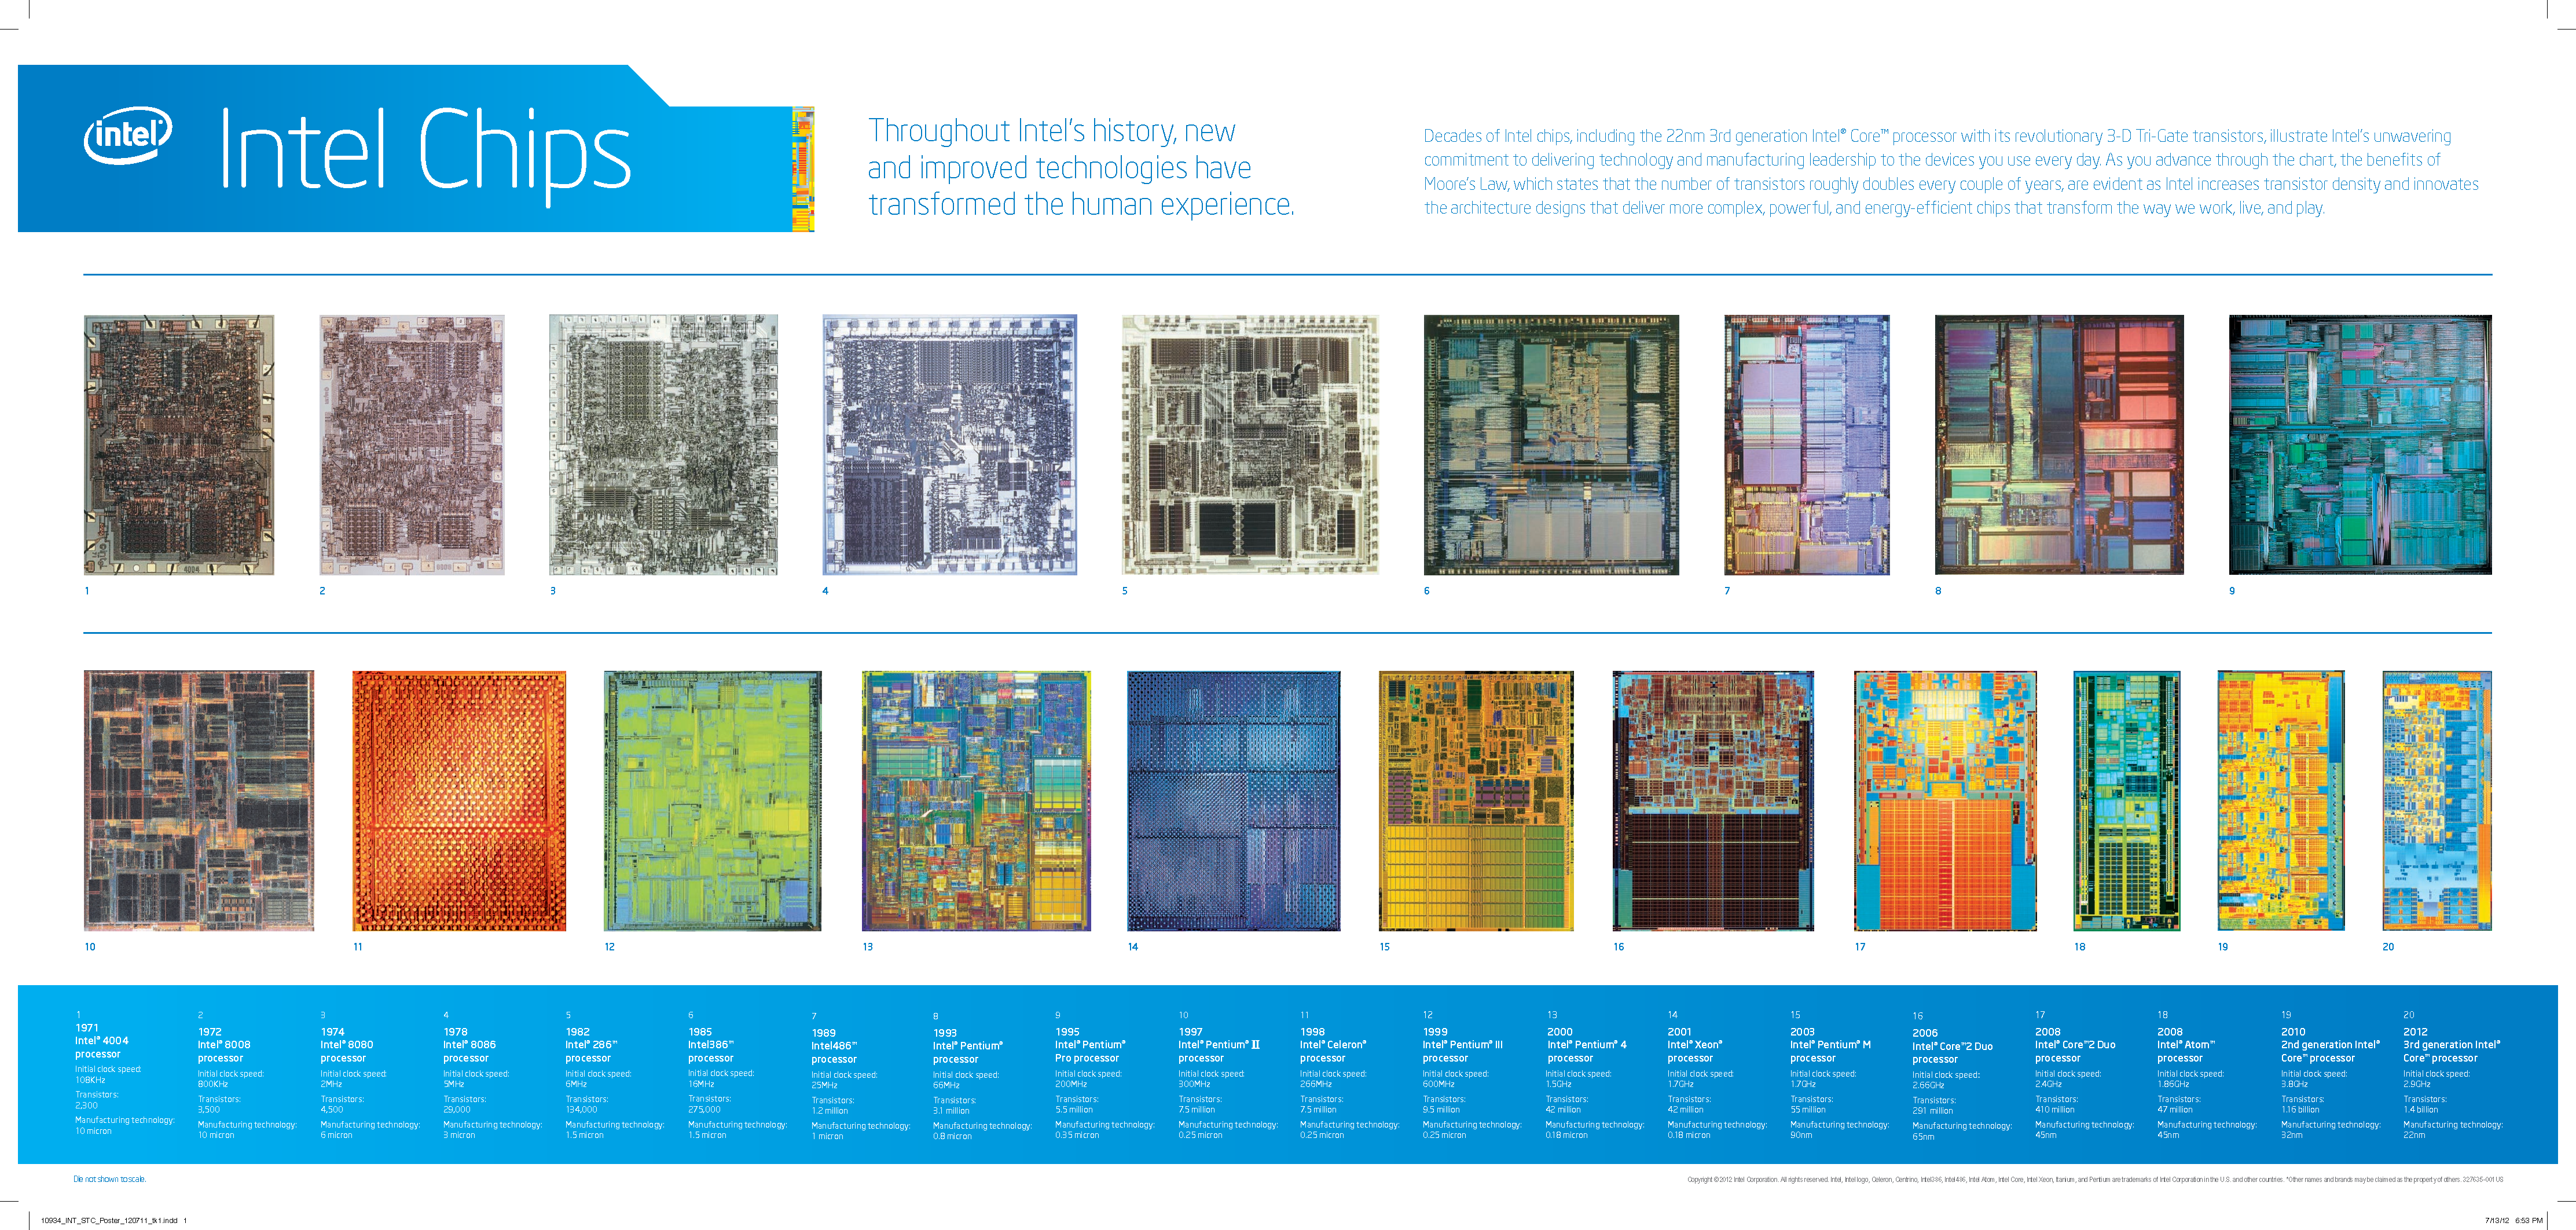
\includegraphics[width=\textwidth]{figure/inteldev.jpg}
        \caption{Intel系列处理器的发展}
    \end{center}
\end{figure}

\subsection{1968-1978 Intel公司的创立与4004处理器的诞生}
\subsubsection{Intel的创立}
1955年,晶体管的发明者威廉·肖克利离开贝尔实验室,创建了肖克利半导体实验室,并且吸引了一大批有才华的年轻科学家加入。但很快,由于内部原因,其中8名科学家联合辞职创办了仙童半导体公司,其中就包括摩尔定律的提出者戈登·摩尔(Gordon Moore)和集成电路的联合发明人罗伯特·诺伊斯(Robert Noyce)。1968年,两人从仙童半导体公司辞职,在7月16日共同创办Intel公司。其名称来源于集成电路(Integrated Electronics)的首字母缩写。
\begin{figure}[H]
    \begin{center}
        
\includegraphics[width=0.2\textwidth]{figure/intel.png}
        \caption{Intel公司现在的logo}
    \end{center}
\end{figure}
起初,Intel的业务主要来自半导体存储器市场,主攻DARM和SARM,在整个20世纪70年代,CPU都不是Intel最主要业务。1971年11月15日,Intel的工程师霍夫(Marcian Hoff)发明了世界上第一块大规模集成电路,也是第一颗微处理器Intel 4004。恐怕那时Intel公司自己也未曾想到,这一天将被永远载入史册,这一“无心之举”也成为了Intel在今后几十年绝大部分的收入来源。

\subsubsection{Intel 4004}
4004处理器起初只是用于在日本Busicom公司生产的计算器中替换一些应用导向集成电路。它只有4位,45条指令,最高主频也仅有740kHz,甚至比不上ENIAC。但由于它集成化程度高,体积小,为个人计算机的发展铺平了道路,具有重要的里程碑意义。
\begin{figure}[H]
    \begin{center}
        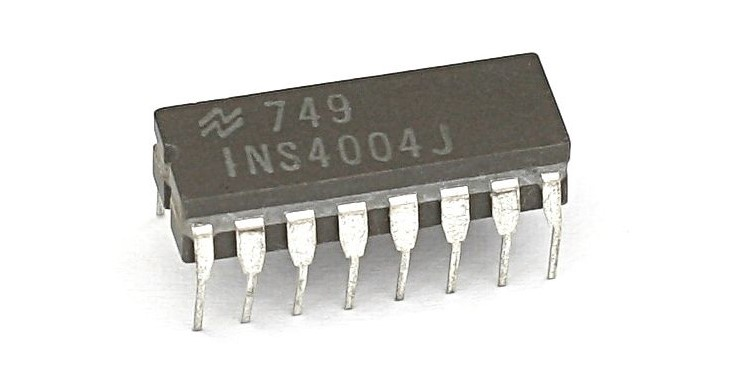
\includegraphics[width=0.4\textwidth]{figure/4004.jpg}
        \caption{Intel 4004}
    \end{center}
\end{figure}

\subsubsection{Intel 8008/8080}
在接下来的几年中,Intel又推出了8位的8008(1972)和8080(1974)处理器。在研发8008的过程中,Intel还获得了由德州的Datapoint公司开发的指令集,正是这套指令集,奠定了今天x86系列指令集的基础。与此同时,微处理器的优势也逐渐被人们所认同。尤其是8080处理器获得了空前的成功。该处理器主频为2MHz,性能是8008的十倍。作为人类历史上的第一台个人计算机Altair也使用了8080处理器作为核心。
\begin{figure}[H]
    \centering
    \subfigure[Intel 8008]{
        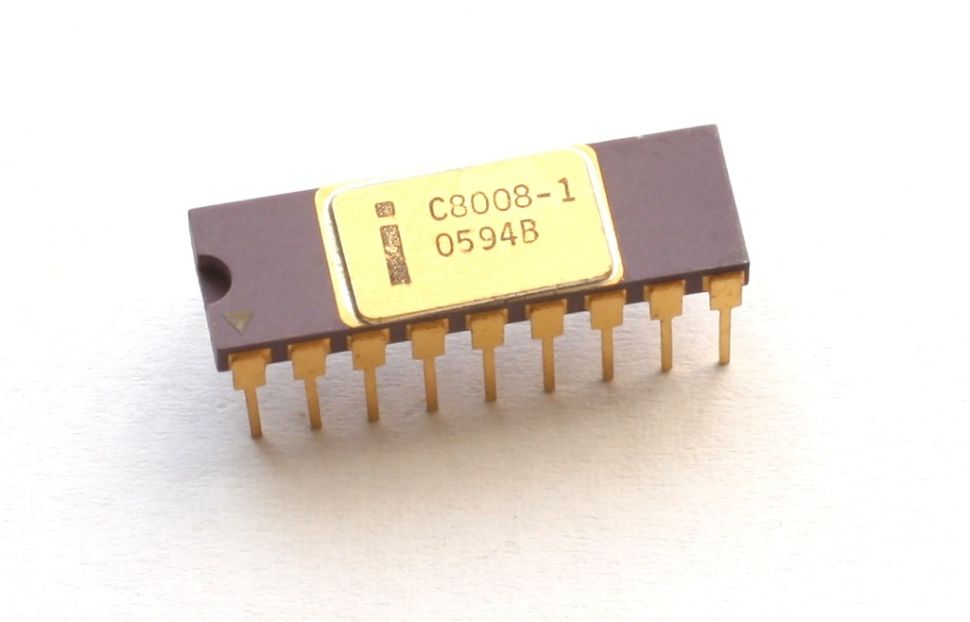
\includegraphics[width=0.5\textwidth]{figure/8008.jpg}
    }
    \subfigure[Intel 8080]{
        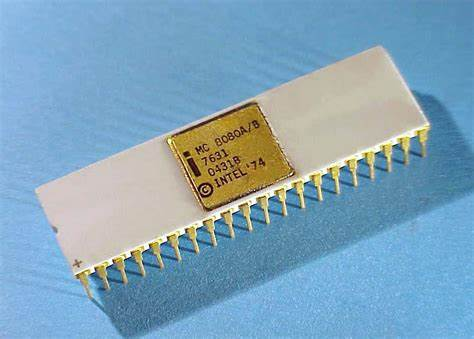
\includegraphics[width=0.4\textwidth]{figure/8080.jpg}
    }
    \caption{Intel 8008/8080}
\end{figure}

\subsection{1978-1993 x86系列处理器与x86指令集的开端}
这一阶段,Intel以8086处理器为开端,开创了x86指令集架构,这一架构也对未来的处理器发展有着深远影响。
\subsubsection{Intel 8086/8088}
1978年,Intel推出了8086处理器。它有16位的数据总线,可一次读取1MB内存,是Intel推出的首个16位处理器。与此同时,Intel还在其上使用了x86指令集。子从那时起,几乎所有的Intel和AMD处理器的指令集都是基于该指令集。从此,x86也成为了个人计算机的标准平台,也是历来最成功的CPU架构之一。

几乎与此同时,Intel也推出了8088处理器,将地址总线提升至20bit。两款处理器都采用了相同的16位x86架构。
\begin{figure}[H]
    \begin{center}
        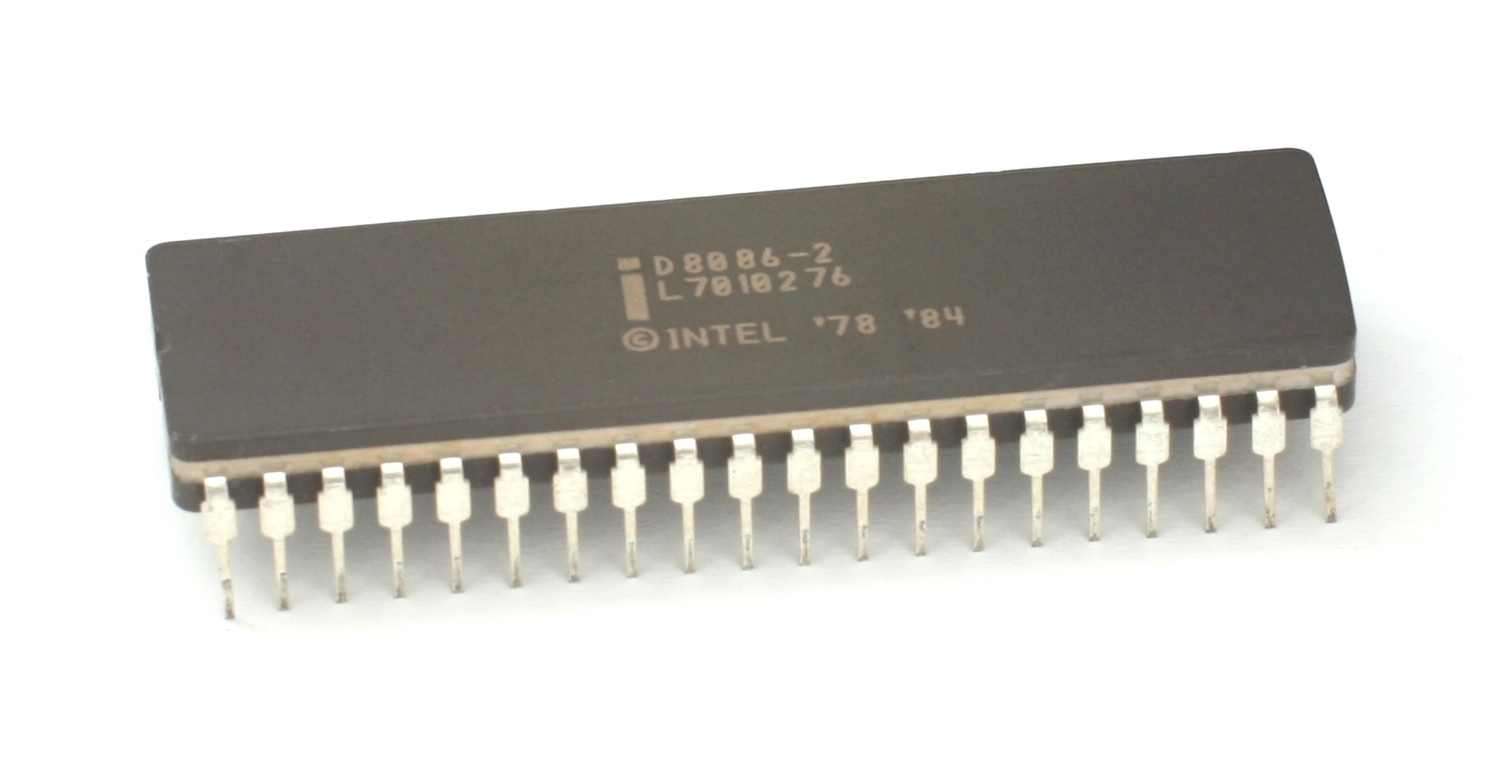
\includegraphics[width=0.3\textwidth]{figure/8086.jpg}
        \caption{Intel 8086}
    \end{center}
\end{figure}

\subsubsection{Intel 80x86系列}
随着PC市场需求的一步步扩大,CPU业务逐渐成为了Intel的主业。从1980年起,Intel接连推出了一系列基于x86架构的处理器,包括80186(1980)、80188(1980)、80286(1982)、80386(1985)和80486(1989)。
\begin{figure}[H]
    \centering
    \subfigure[Intel 80186]{
        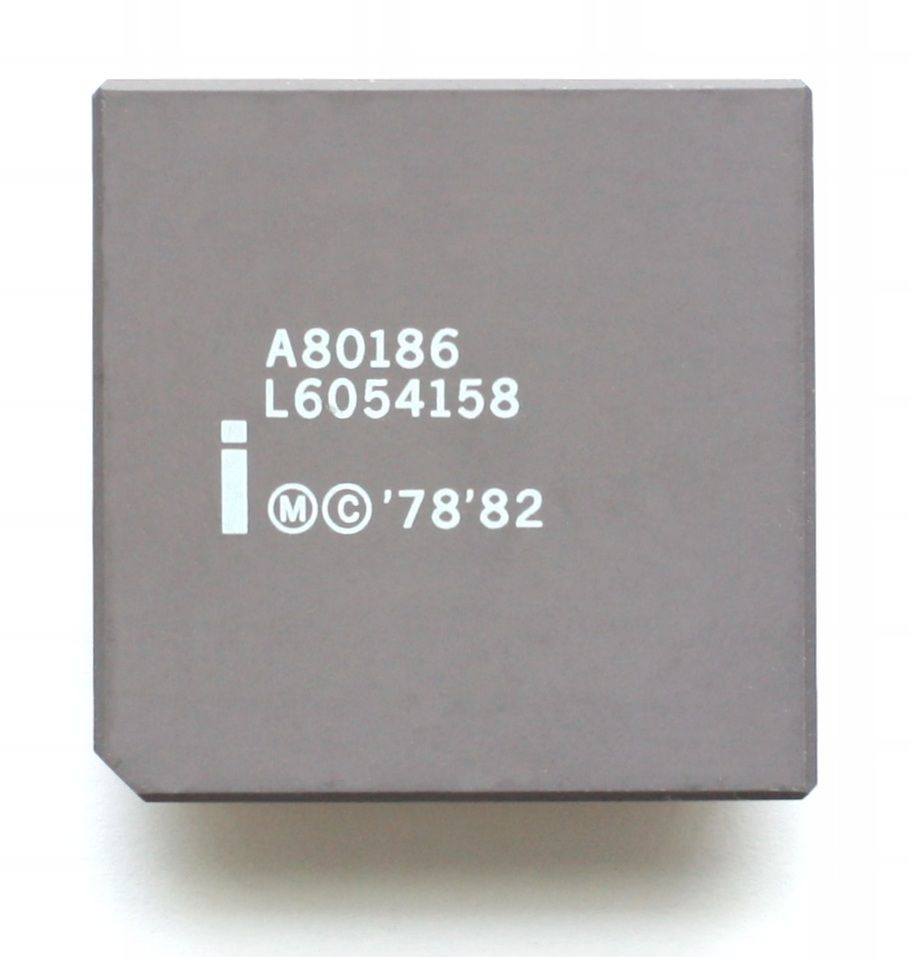
\includegraphics[width=0.3\textwidth]{figure/80186.jpg}
    }
    \subfigure[Intel 80486]{
        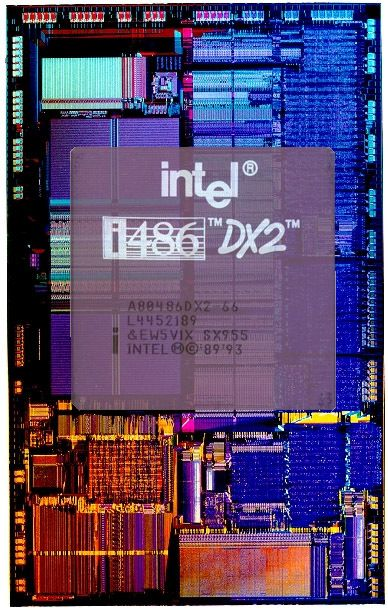
\includegraphics[width=0.2\textwidth]{figure/80486.jpg}
    }
    \caption{Intel 80186和80486}
\end{figure}
其中,80188和80186几乎同时推出,80188削减了一半的外部数据总线以降低成本。80286是Intel第一款完全兼容前代CPU的处理器。

从1985年的80386开始,Intel系列处理器进入32位时代,32位的x86架构也称为IA-32。80386集成了27万多只晶体管,规模超过了了初代CPU 4004的100倍,同时也是第一款具有多任务功能的处理器,这也为操作系统的发展有重要影响。

1989年,Intel发布了最后一款用数字命名的处理器——Intel 80486。在这一代CPU上,Intel首次将FPU(浮点计算单元)集成在CPU之内。此外,8KB的L1缓存第一次出现在了x86 CPU上。


\subsection{1993-2006 奔腾(Pentium)时代}
经过一系列80x86处理器,Intel已经从一家主攻存储芯片的公司,转为CPU领域的霸主。1993年,Intel发布了以子商标奔腾(Pentium)命名的处理器,正式宣告处理器进入奔腾时代。
\subsubsection{Pentium与Pentium MMX}
1993年,采用P5架构的Pentium处理器发布,而没有遵循80x86号码系统。这是一个划时代的事件。在接下来的十几年间,奔腾几乎成为了家喻户晓的名字,时至今日仍在使用。初代Pentium系列将CPU的工作电压降至3.3V,增强了浮点数的运算,新使用的P5架构使得它在所有方面都比80486快。1994年,Pentium处理器被发现在浮点数的计算上出现了瑕疵,Intel不得不召回大批的Pentium处理器。

然而这一事件并未影响Intel在CPU领域的高歌猛进。1996年,主攻服务器方向,采用P6架构的Pentium Pro推出。1997年1月,Pentium MMX推出。它扩展了L1缓存至16KB,也扩展了新的MMX指令集,使得其对多媒体数据的处理更为强大,也因此红极一时。此外,MMX系列的处理器还拥有较强的超频能力,还能通过提高其核心电压来获得更好的性能。1997年,同样采用P6架构的Pentium \uppercase\expandafter{\romannumeral2}发布,L1缓存已经增加到16KB数据缓存+16KB指令缓存共32KB。
\begin{figure}[H]
    \centering
    \subfigure[Pentium MMX]{
        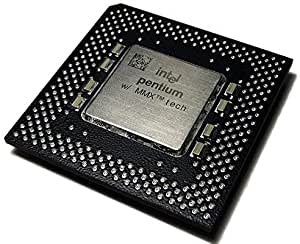
\includegraphics[width=0.25\textwidth]{figure/pentium.jpg}
    }
    \subfigure[Pentium Pro]{
        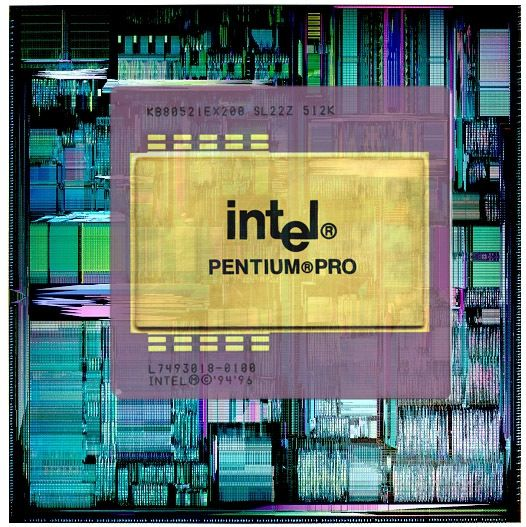
\includegraphics[width=0.2\textwidth]{figure/pentium_pro.jpg}
    }
    \caption{Pentium和Pentium Pro}
\end{figure}

\subsubsection{赛扬(Celeron)和至强(Xeon)}
1998年,随着AMD大举入侵低价处理器市场,而同期的Pentium \uppercase\expandafter{\romannumeral2}价格昂贵。为了兼顾低端市场,Intel将Pentium \uppercase\expandafter{\romannumeral2}中的两颗L2缓存取消,推出了初代Celeron处理器,从此诞生了“赛扬”这一新的产品线。

同时,为区分服务器市场与PC市场,英特尔还推出了Pentium \uppercase\expandafter{\romannumeral2} Xeon作为Pentium Pro的升级产品,从此诞生了Xeon处理器。直到2001年,Intel将Xeon系列前面的Pentium取消,从此独立出面向中高端服务器市场的Xeon系列。

时至今日,Celeron和Xeon系列仍然是Intel CPU中最低端和高端的代表。而它们都脱胎于当年的Pentium系列。
\begin{figure}[H]
    \centering
    \subfigure[Celeron]{
        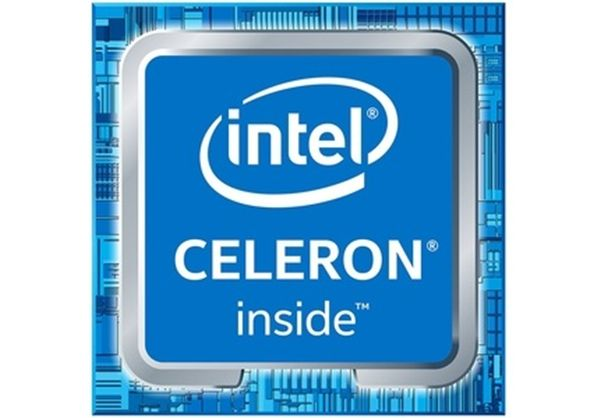
\includegraphics[width=0.3\textwidth]{figure/celeron.jpg}
    }
    \subfigure[Xeon]{
        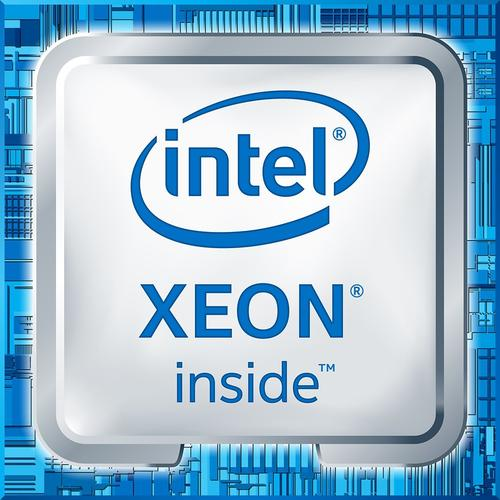
\includegraphics[width=0.21\textwidth]{figure/xeon.jpg}
    }
    \caption{Celeron和Xeon系列}
\end{figure}

\subsubsection{Pentium系列的后续产品}
世纪之交,Pentium系列产品的更新迭代还在继续。Intel相继推出了Pentium \uppercase\expandafter{\romannumeral3}(1999)、Pentium 4(2000)、Pentium M(2004)和Pentium D处理器。

其中,1999年推出的Pentium \uppercase\expandafter{\romannumeral3}处理器的主频首次突破1GHz。2002年,Intel在Pentium 4上首次运用了超线程技术。2005年,带有两个处理器内核的Pentium D推出,开启了CPU多内核的时代。以上三点是Pentium系列在这几年中主要的创新点。

然而在这一时期,从Pentium 4开始使用的P4架构“Netburst”出现了功耗和热量问题,在很长一段时间内,Intel无法将Netburst架构的处理器主频升至2GHz以上。随后,在此基础上改进的“Prescott”架构(被用于Pentium D)同样也出现了类似的问题。在一段短暂的时间中,Intel的在CPU领域的统治被AMD所打破。这也迫使Intel放弃Netburst架构,转而支持基于P6的Pentium M设计,这也促成了Intel新一代产品酷睿(Core)的诞生。

\subsection{2006-至今 酷睿(Core)的又一次辉煌}
随着AMD的步步紧逼,Intel不得不调整自己的策略。从2005年开始,Intel制定了一套“钟摆计划”(Tick-Tock),并在2006年推出了新一代酷睿(Core)产品,重新逆转了与AMD的竞争局面。时至今日,Core系列产品仍是广大消费者选择CPU的不二之选。
\subsubsection{Core 2 Duo:初代Core}
从2004到2006,Intel陷入了一段低迷时期。AMD凭借其K8系列,以“真双核”和较好的能效比赚足了世人的眼球。为了从AMD手中重新夺回CPU市场的主导地位,Intel启动了Tick-Tock计划,即用时钟的声响(Tick,Tock为拟声词)代表芯片制程和处理器微架构的更新。2005年,Core一代产品发布,标志这Core系列处理器的诞生。此时的Core,架构源自Pentium M,而新架构的开山之作,即是2006年7月发布的Core 2 Duo。
\begin{figure}[H]
    \centering
    \subfigure[]{
        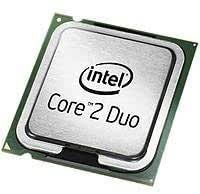
\includegraphics[width=0.2\textwidth]{figure/core2duo.jpg}
    }
    \subfigure[]{
        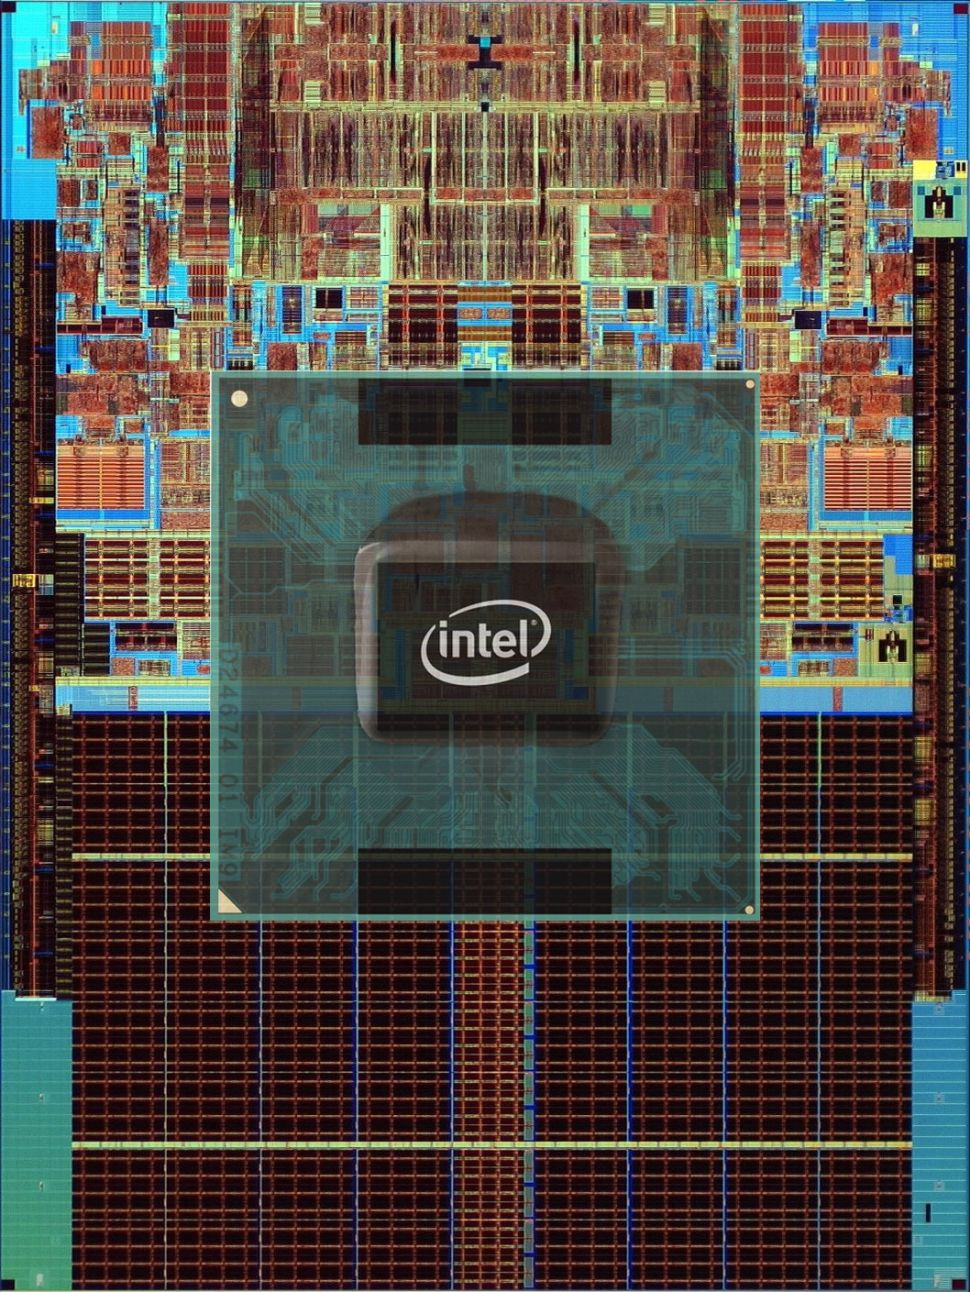
\includegraphics[width=0.15\textwidth]{figure/core2duoin.jpg}
    }
    \caption{Core 2 Duo}
\end{figure}

Core 2 Duo采用了65nm制程工艺,Intel声称它对比上一代产品有40\%的性能提升,同时减少40\%的功耗,各项数据均大幅领先当时AMD的Athlon 64X2。从此,Intel再次夺回了CPU的主导权。

究其原因,Core 2 Duo抛弃了此前出现各种问题的Netburst架构,转而对Pentium M的微架构进行改进,定名Core架构。Core 2 Duo为双核心64位处理器,将双核共享的L2缓存提升至4MB,晶体管总数达到近3亿个,此外还加入了对EM64T与SSE4指令集的支持,使其拥有更强大的寻址空间。Core微架构的改进,实现了能效比的大幅提升。

此后,由于Core架构的巨大成功,Intel将其也运用到了Celeron、Pentium乃至Xeon产品线中。

\subsubsection{i系列处理器:更清晰的产品定位}
随着Core 2 Duo的发布,Intel的优势再一次被确立,在随后的几年中,Tick-Tock战略稳步实施。2008年,Intel推出的新的Nehalem微架构,引入了新的命名方案。共有三个变体,Core i3,Core i5和Core i7。2008年11月17日,Intel推出了四核的Core i7处理器。2009年9月8日,第一款Core i5发布。2010年1月7日,首款Core i3发布。i3,i5和i7分别针对入门级消费者,普通消费者和高端消费者,但不再以核心数等技术指标命名。
\begin{figure}[H]
    \begin{center}
        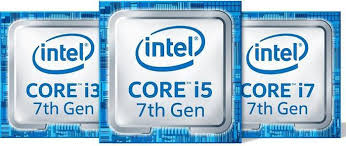
\includegraphics[width=0.4\textwidth]{figure/core1.jpg}
        \caption{Intel Core i系列}
    \end{center}
\end{figure}

在此后的几年中,Intel的i系列处理器陆续推出了一代(Nehalem微架构,45nm,2008),二代(Sandy Bridge微架构,32nm,2011),三代(Ivy Bridge微架构,22nm,2012),四代(Haxwell微架构,22nm,2013)处理器。随着制程和微架构的提升,Core处理器的性能也稳步提升。其中有几个比较有突破性的进展:在Core一代中的部分处理器首次集成了图形处理单元(GPU),Core i7在2010年首次发布了六核处理器,Core二代产品首次支持高性能DDR3内存等。经过几年的产品迭代改进,Intel Core系列在消费级CPU中已经形成了一家独大的局面。

\subsubsection{14nm的爆发}
2015年,CPU制程已经提升至14nm,intel也发布了基于14nm制程的Broadwell微架构的第五代Core处理器。这一代产品的高端型号甚至出现了8核甚至10核的夸张表现。此后发布的第六代(Skylake,2015),第七代(Kaby Lake,2016),第八代(Coffee Lake,2017/Whiskey Lake,2018),第九代(Coffee Lake,2018)Core处理器同样基于14nm制程。

在此期间,Intel两次提升了台式机处理器中的CPU核心数和线程数。在2017年5月,还发布了全新的Core i9系列,作为Core系列的旗舰产品。
\begin{figure}[H]
    \centering
    \subfigure[Intel Core i9]{
        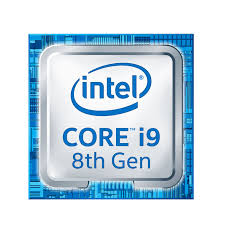
\includegraphics[width=0.2\textwidth]{figure/corei9.jpg}
    }
    \subfigure[Intel Core 10th gen]{
        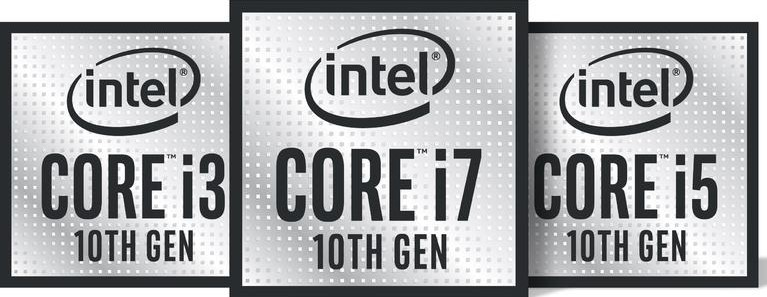
\includegraphics[width=0.5\textwidth]{figure/core10.jpg}
    }
\end{figure}


2019年,Core系列最新一代产品Core十代处理器发布,包括部分基于10nm制程,Comet Lake架构的处理器。Intel的处理器制程第一次突破了14nm。
\begin{table}[H]
    \centering
    \caption{Intel核心数与线程数的发展}
    \begin{tabular}{cccc}
        \toprule
        型号    & 第七代 & 第八代 & 第九代 \\
        \midrule
        Core i3 & 2C/4T  & 4C/4T  & 4C/4T  \\
        Core i5 & 4C/4T  & 6C/6T  & 6C/6T  \\
        Core i7 & 4C/8T  & 6C/12T & 8C/8T  \\
        Core i9 & /      & /      & 8C/16T\\
        \bottomrule
    \end{tabular}
\end{table}
\newpage






\section{AMD系列处理器发展历程}
\subsection{1969-1996 AMD公司的创立和Intel的代工厂}
\subsection{1996-1999 K5和K6:自研CPU的初尝试}
\subsection{1999-2006 K7到Athlon 64X2 AMD的崛起和辉煌}
\subsection{2006-2017 AMD失落的十年}
\subsection{2017-至今 锐龙(Ryzen)架构与AMD的重生}
%正文
\end{document}
